\section{Relation and Digraphs}
\subsection{Introduction to binary relations}

A \textbf{Binary Relation} between two sets $A$ and $B$ is a subset $R$ of $A \times B$.
It is binary because it is between two sets.
\[
  \text{for } a \in A \land b \in B, (a,b) \in R \text{ is denoted as } a\text{R}b
\]

For example, consider the relation C between $\mathbb{R}$ and $\mathbb{Z}$:
\[
  x\text{C}y \text{ if } \left\lvert x-y\right\rvert \leq 1, \text{ where } x \in \mathbb{R} \text{ and } y \in \mathbb{Z}
\]
If $A$ and $B$ are finite, then relation R between $A$ and $B$ can be represented by a set of ordered pairs.

\subsubsection*{Matrix Representation}
\begin{align*}
  P           & = \{\text{Sue}, \text{Harry}, \text{Sam}\}                       \\
  \text{File} & = \{\text{File A}, \text{File B}, \text{File C}, \text{File D}\}
\end{align*}
\[
  \bordermatrix{ & \text{File A} & \text{File B} & \text{File C} & \text{File D} \cr
    \text{Sue}   & 0 & 1 & 1 & 1 \cr
    \text{Harry} & 1 & 0 & 0 & 0 \cr
    \text{Sam}   & 0 & 0 & 0 & 0 \cr }
\]
\begin{center}
  An element is
  \begin{tabular}{c}
    1 if $p$R$f$ is true \\
    0 if $p$R$f$ is false
  \end{tabular}
\end{center}

\subsubsection*{Arrow Diagram}
\begin{align*}
  A & = \{a,b,c,d,e\}                                \\
  R & \subseteq A \times A                           \\
  R & = \{(a,b), (b,c), (e,c), (c,e), (d,a), (d,d)\}
\end{align*}
\begin{center}
  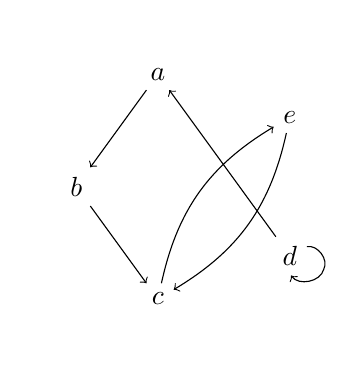
\begin{tikzpicture}
    %VARIABLES
    \pgfmathsetmacro{\gsize}{1.5}
    \pgfmathsetmacro{\gnum}{5}

    \foreach[count=\i] \element in {a,b,c,d,e} { %domain
        \node (\element) at (\i * 360 / \gnum + 180 / \gnum:\gsize) {$\element$};
        \node (\element-) at (\i * 360 / \gnum + 180 / \gnum:\gsize + 0.5) {};
      }
    \foreach \j/\l in {a/b,b/c,d/a} { %a to b
        \draw[->] (\j) -- (\l);
      }
    \foreach \j/\l in {e/c} { %a to b AND b to a
        \draw[->] (\j) to[bend left=20 / \gsize + 10] (\l);
        \draw[->] (\l) to[bend left=20 / \gsize + 10] (\j);
      }
    \foreach \j in {d} { %a to a
        \draw[->] (\j) to[bend left=65] (\j-)
        to[bend left=65] (\j);
      }
  \end{tikzpicture}
\end{center}

\subsubsection*{Arrow Diagram vs. Matrix Representation}
\begin{align*}
  A & = \{1,2,3,4\}                                  \\
  R & = \{(1,2), (1,3), (2,2), (2,3), (3,4), (4,3)\}
\end{align*}
\begin{center}
  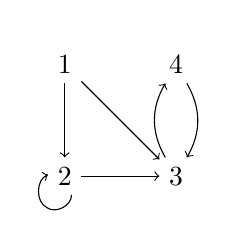
\begin{tikzpicture}
    %VARIABLES
    \pgfmathsetmacro{\gsize}{1}
    \pgfmathsetmacro{\gnum}{4}

    \foreach[count=\i] \element in {1,2,3,4} { %domain
        \node (\element) at (\i * 360 / \gnum + 180 / \gnum:\gsize) {$\element$};
        \node (\element-) at (\i * 360 / \gnum + 180 / \gnum:\gsize + 0.5) {};
      }
    \foreach \j/\l in {1/2,1/3,2/3} { %a to b
        \draw[->] (\j) -- (\l);
      }
    \foreach \j/\l in {3/4} { %a to b AND b to a
        \draw[->] (\j) to[bend left=20 / \gsize + 10] (\l);
        \draw[->] (\l) to[bend left=20 / \gsize + 10] (\j);
      }
    \foreach \j in {2} { %a to a
        \draw[->] (\j) to[bend left=65] (\j-)
        to[bend left=65] (\j);
      }
  \end{tikzpicture}
  \qquad
  $
    \bordermatrix{ & 1 & 2 & 3 & 4 \cr
      1 & 0 & 1 & 1 & 0 \cr
      2 & 0 & 1 & 1 & 0 \cr
      3 & 0 & 0 & 0 & 1 \cr
      4 & 0 & 0 & 1 & 0 \cr }
  $
\end{center}

\subsection{Properties of binary relations}

A binary relation of R on set $A$ is \textbf{Reflective} if for \textit{every} $x \in A$, $x$R$x$.
For Arrow Diagrams, this means the graph contains self-loops:
\begin{center}
  \begin{tikzpicture}
    %VARIABLES
    \pgfmathsetmacro{\gsize}{1}
    \pgfmathsetmacro{\gnum}{2}

    \foreach[count=\i] \element in {a,b} { %domain
        \node (\element) at (\i * 360 / \gnum:\gsize) {$\element$};
        \node (\element-) at (\i * 360 / \gnum:\gsize + 0.5) {};
      }
    \foreach \j in {a,b} { %a to a
        \draw[->] (\j) to[bend left=65] (\j-)
        to[bend left=65] (\j);
      }
  \end{tikzpicture}
\end{center}
For Matrix Representation, this means that the top left to bottom right diagonal are all 1's:
\[
  \bordermatrix{ & a & b & c & d \cr
    a & 1 & - & - & - \cr
    b & - & 1 & - & - \cr
    c & - & - & 1 & - \cr
    d & - & - & - & 1 \cr }
\]

A binary relation of R on set $A$ is \textbf{Anti-reflective} if for \textit{every} $x \in A$, $x$R$x$ is \textit{not} true.
For Arrow Diagrams, this means the graph does not contain self-loops:
\begin{center}
  \begin{tikzpicture}
    %VARIABLES
    \pgfmathsetmacro{\gsize}{1}
    \pgfmathsetmacro{\gnum}{2}

    \foreach[count=\i] \element in {a,b} { %domain
        \node (\element) at (\i * 360 / \gnum:\gsize) {$\element$};
        \node (\element-) at (\i * 360 / \gnum:\gsize + 0.5) {};
      }
  \end{tikzpicture}
\end{center}
For Matrix Representation, this means that the top left to bottom right diagonal are all 0's:
\[
  \bordermatrix{ & a & b & c & d \cr
    a & 0 & - & - & - \cr
    b & - & 0 & - & - \cr
    c & - & - & 0 & - \cr
    d & - & - & - & 0 \cr }
\]

A binary relation of R on set $A$ is \textbf{Symmetric} if and only if for \textit{every} pair $x \in A$, $y \in Y$,
either \textit{both} $x$R$y$ \underline{and} $y$R$x$, or \textit{both} not $x$R$y$ or not $y$R$x$ is true.
For Arrow Diagrams, this means that every arrow has an arrow going the other way:
\begin{center}
  \begin{tikzpicture}
    %VARIABLES
    \pgfmathsetmacro{\gsize}{1}
    \pgfmathsetmacro{\gnum}{4}

    \foreach[count=\i] \element in {a,b,c} { %domain
        \node (\element) at (\i * 360 / \gnum:\gsize) {$\element$};
        \node (\element-) at (\i * 360 / \gnum:\gsize + 0.5) {};
      }
    \foreach \j/\l in {a/b,b/c} { %a to b AND b to a
        \draw[->] (\j) to[bend left=20 / \gsize + 10] (\l);
        \draw[->] (\l) to[bend left=20 / \gsize + 10] (\j);
      }
  \end{tikzpicture}
\end{center}
For Matrix Representation, this means that the matrix is symmetric along the top left to bottom right diagonal:
\begin{center}
  $
    \bordermatrix{ & a & b & c & d \cr
      a & - & u & v & x \cr
      b & u & - & w & y \cr
      c & v & w & - & z \cr
      d & x & y & z & - \cr }
  $
  where
  \begin{tabular}{c}
    $u \in \{0,1\}$ \\
    $\vdots$        \\
    $z \in \{0,1\}$
  \end{tabular}
\end{center}

A binary relation of R on set $A$ is \textbf{Anti-symmetric} if and only if for \textit{every} pair $x \in A$, $y \in Y$, $x$R$y$ xor $y$R$x$.
For Arrow Diagrams, this means that each arrow does not have an arrow going the other way:
\begin{center}
  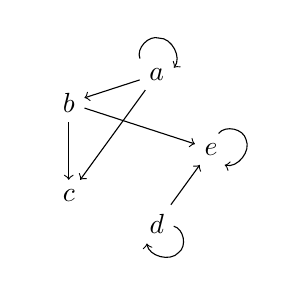
\begin{tikzpicture}
    %VARIABLES
    \pgfmathsetmacro{\gsize}{1}
    \pgfmathsetmacro{\gnum}{5}

    \foreach[count=\i] \element in {a,b,c,d,e} { %domain
        \node (\element) at (\i * 360 / \gnum:\gsize) {$\element$};
        \node (\element-) at (\i * 360 / \gnum:\gsize + 0.5) {};
      }
    \foreach \j/\l in {a/b, b/c, a/c, b/e, d/e} { %a to b
        \draw[->] (\j) -- (\l);
      }
    \foreach \j in {a,e,d} { %a to a
        \draw[->] (\j) to[bend left=65] (\j-)
        to[bend left=65] (\j);
      }
  \end{tikzpicture}
\end{center}
For Matrix Representation, this means that the matrix is anti-symmetric along the top left to bottom right diagonal:
\begin{center}
  $
    \bordermatrix{ & a & b & c & d \cr
      a & - & \bar{u} & \bar{v} & \bar{x} \cr
      b & u & - & \bar{w} & \bar{y} \cr
      c & v & w & - & \bar{z} \cr
      d & x & y & z & - \cr }
  $
  where
  \begin{tabular}{c}
    $u \in \{0,1\}$ \\
    $\vdots$        \\
    $z \in \{0,1\}$
  \end{tabular}
\end{center}

A binary relation of R on set $A$ is \textbf{Transitive} if for \textit{every} three elements $x,y,z \in A$,
if $x$R$y$ and $y$R$z$, then $x$R$z$. Logically, ($x$R$y \land y$R$z) \implies x$R$z$.
For Arrow Diagrams, this means the graph follows a hierarchy or kind of flow:
\begin{center}
  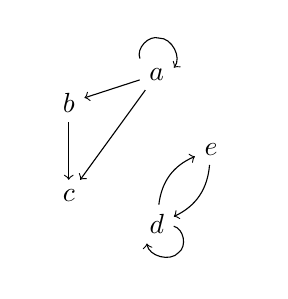
\begin{tikzpicture}
    %VARIABLES
    \pgfmathsetmacro{\gsize}{1}
    \pgfmathsetmacro{\gnum}{5}

    \foreach[count=\i] \element in {a,b,c,d,e} { %domain
        \node (\element) at (\i * 360 / \gnum:\gsize) {$\element$};
        \node (\element-) at (\i * 360 / \gnum:\gsize + 0.5) {};
      }
    \foreach \j/\l in {a/b,b/c,a/c} { %a to b
        \draw[->] (\j) -- (\l);
      }
    \foreach \j/\l in {d/e} { %a to b AND b to a
        \draw[->] (\j) to[bend left=20 / \gsize + 10] (\l);
        \draw[->] (\l) to[bend left=20 / \gsize + 10] (\j);
      }
    \foreach \j in {d,a} { %a to a
        \draw[->] (\j) to[bend left=65] (\j-)
        to[bend left=65] (\j);
      }
  \end{tikzpicture}
\end{center}
For Matrix Representation, it is much more difficult to determine transitivity, but here is an example:
\[
  \bordermatrix{ & a & b & c & d & e \cr
    a & 1 & 1 & 1 & 0 & 0 \cr
    b & 0 & 0 & 1 & 0 & 0 \cr
    c & 0 & 0 & 0 & 0 & 0 \cr
    d & 0 & 0 & 0 & 1 & 1 \cr
    e & 0 & 0 & 0 & 1 & 0 \cr }
\]

\subsection{Directed graphs, paths, and cycles}

A directed graph, or \textbf{Diagraph}, consists of a pair $(V,E)$, where $V$ is the set of vertices
and $E$ is the set of \textit{directed edges}. It is a subset of $V \times V$.
\begin{itemize}
  \item indegree: \# of edges pointing towards a vertex, $\text{indegree}(u) = \left\lvert\{v : (v,u) \in E\}\right\rvert$
  \item outdegree: \# of edges pointing away from a vertex, $\text{outdegree}(u) = \left\lvert\{u : (v,u) \in E\}\right\rvert$
\end{itemize}
A digraph is organized into a cartesian pair of the set of vertices and edge pairs:
\begin{align*}
  \text{Graph } G & = (V,E)                      \\
  V               & = \{a,b,c,d\}                \\
  E               & = \{(a,b),(b,c)(a,c),(d,d)\}
\end{align*}
\begin{center}
  \begin{tikzpicture}
    %VARIABLES
    \pgfmathsetmacro{\gsize}{1}
    \pgfmathsetmacro{\gnum}{4}

    \foreach[count=\i] \element in {a,b,c,d} { %domain
        \node (\element) at (\i * 360 / \gnum:\gsize) {$\element$};
        \node (\element-) at (\i * 360 / \gnum:\gsize + 0.5) {};
      }
    \foreach \j/\l in {a/b,b/c,a/c} { %a to b
        \draw[->] (\j) -- (\l);
      }
    \foreach \j/\l in {} { %a to b AND b to a
        \draw[->] (\j) to[bend left=20 / \gsize + 10] (\l);
        \draw[->] (\l) to[bend left=20 / \gsize + 10] (\j);
      }
    \foreach \j in {d} { %a to a
        \draw[->] (\j) to[bend left=65] (\j-)
        to[bend left=65] (\j);
      }
  \end{tikzpicture}
\end{center}
\begin{align*}
  \text{indegree}(c) & = 2 & \text{outdegree}(a) & = 2 & a & \text{ is the \underline{tail} of edge $(a,b)$} \\
  \text{indegree}(d) & = 1 & \text{outdegree}(d) & = 1 & b & \text{ is the \underline{head} of edge $(a,b)$} \\
\end{align*}

A digraph is mathematically the same as a relation. Here is an example of the internet as a graph:
\begin{align*}
  \text{Graph } G & = (V,E)                                                     \\
  V               & = \text{ set of all URLs}                                   \\
  E               & = \text{ set of all hyperlinks from one URL to another URL}
\end{align*}
\begin{align*}
  B   & = \text{ Blog}                   \\
  P   & = \text{ Pediatrician website}   \\
  PC  & = \text{ Pharmaceutical Company} \\
  AoP & = \text{ Academy of Pediatrics}
\end{align*}
\begin{center}
  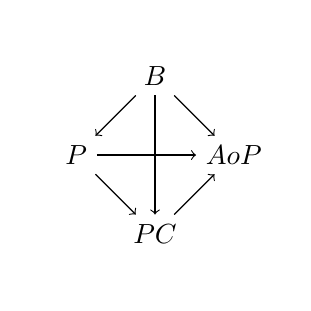
\begin{tikzpicture}
    %VARIABLES
    \pgfmathsetmacro{\gsize}{1}
    \pgfmathsetmacro{\gnum}{4}

    \foreach[count=\i] \element in {B, P, PC, AoP} { %domain
        \node (\element) at (\i * 360 / \gnum:\gsize) {$\element$};
        \node (\element-) at (\i * 360 / \gnum:\gsize + 0.5) {};
      }
    \foreach \j/\l in {B/P, B/PC, B/AoP, P/PC, P/AoP, PC/AoP} { %a to b
        \draw[->] (\j) -- (\l);
      }
    \foreach \j/\l in {} { %a to b AND b to a
        \draw[->] (\j) to[bend left=20 / \gsize + 10] (\l);
        \draw[->] (\l) to[bend left=20 / \gsize + 10] (\j);
      }
    \foreach \j in {} { %a to a
        \draw[->] (\j) to[bend left=65] (\j-)
        to[bend left=65] (\j);
      }
  \end{tikzpicture}
\end{center}

\subsubsection*{Walks in Directed Graphs}

A \textit{walk} is a sequence of vertices and edges. For example, a walk from $v_0$ to $v_l$ is notated as:
\[
  \left\langle v_0,(v_0,v_1), v_1,(v_1,v_2), \ldots,(v_{l-1},v_l), v_l\right\rangle
\]
where each edge in the sequence appears after its tail and before its head. A walk can also be a set of vertices:
\[
  \left\langle v_0, v_1, \ldots, v_l\right\rangle
\]
provided that the edges between the vertices \textit{actually exist}.
The \textbf{length} of a walk is the number of edges traversed.
\begin{itemize}
  \item \textbf{Open walk}: first and last vertices are \textit{not} the same
  \item \textbf{Closed walk}: first and last vertices \textit{are} the same.
\end{itemize}

\subsubsection*{Trails, Circuits, Paths, Cycles}
\begin{itemize}
  \item \textbf{Trail}: \textit{open} walk in which no edge occurs more than once.
  \item \textbf{Circuit}: \textit{closed} walk in which no edge occurs more than once. A circuit is a closed trail.
  \item \textbf{Path}: \textit{trail} where no vertex occurs more than once.
  \item \textbf{Cycle}: \textit{circuit} where no vertex occurs more than once, \textit{except} for the first and last, which are the same.
\end{itemize}
Here are some examples:
\begin{align*}
  \left\langle a,c,d,a\right\rangle   & \text{ is a \textbf{cycle}: only the first and last vertices are repeated.} \\
  \left\langle a,c,a,d,a\right\rangle & \text{ is a \textbf{circuit}: vertices are repeated, but not edges}         \\
  \left\langle a,b,c,b,d\right\rangle & \text{ is a \textbf{trail}: open, vertices are repeated, but not edges}
\end{align*}

\subsection{Composition of relations}

\begin{itemize}
  \item one-to-one correspondence between digraphs and binary relations
  \item arrow diagram for a binary relation \textit{is} a directed graph
\end{itemize}
The \textbf{composition} of relations R and S on set $A$ is denoted as S$\circ$R. Logically, this is what is means:
\[
  (a,c) \in S \circ R \iff \exists b : (b \in A \land (a,b) \in R \land (b,c) \in S)
\]
Composition is applied \textit{right to left}, much like composition of functions, or matrix transformations.
Therefore, S$\circ$R means R is applied first, then S.
\begin{center}
  \begin{tikzpicture}
    %VARIABLES
    \pgfmathsetmacro{\gsize}{1};
    \pgfmathsetmacro{\gnum}{4};


    \foreach[count=\i] \element in {a,b,c,d} { %domain
        \node (\element) at (\i * 360 / \gnum:\gsize) {$\element$};
        \node (\element-) at (\i * 360 / \gnum:\gsize + 0.5) {};
      }
    \foreach \j/\l in {a/d,b/c} { %a to b
        \draw[->] (\j) -- (\l);
      }
    \foreach \j/\l in {c/d} { %a to b AND b to a
        \draw[->] (\j) to[bend left=20 / \gsize + 10] (\l);
        \draw[->] (\l) to[bend left=20 / \gsize + 10] (\j);
      }
    \foreach \j in {b} { %a to a
        \draw[->] (\j) to[bend left=65] (\j-)
        to[bend left=65] (\j);
      }
    \node[anchor=east] (name) at (145:\gsize+.5) {R}; %relation name
  \end{tikzpicture}
  \qquad
  \begin{tikzpicture}
    %VARIABLES
    \pgfmathsetmacro{\gsize}{1};
    \pgfmathsetmacro{\gnum}{4};


    \foreach[count=\i] \element in {a,b,c,d} { %domain
        \node (\element) at (\i * 360 / \gnum:\gsize) {$\element$};
        \node (\element-) at (\i * 360 / \gnum:\gsize + 0.5) {};
      }
    \foreach \j/\l in {b/a,b/d,d/c} { %a to b
        \draw[->] (\j) -- (\l);
      }
    \foreach \j/\l in {} { %a to b AND b to a
        \draw[->] (\j) to[bend left=20 / \gsize + 10] (\l);
        \draw[->] (\l) to[bend left=20 / \gsize + 10] (\j);
      }
    \foreach \j in {} { %a to a
        \draw[->] (\j) to[bend left=65] (\j-)
        to[bend left=65] (\j);
      }
    \node[anchor=east] (name) at (145:\gsize+.5) {S}; %relation name
  \end{tikzpicture}
  \qquad
  \begin{tikzpicture}
    %VARIABLES
    \pgfmathsetmacro{\gsize}{1};
    \pgfmathsetmacro{\gnum}{4};


    \foreach[count=\i] \element in {a,b,c,d} { %domain
        \node (\element) at (\i * 360 / \gnum:\gsize) {$\element$};
        \node (\element-) at (\i * 360 / \gnum:\gsize + 0.5) {};
      }
    \foreach \j/\l in {a/c,b/a,b/d} { %a to b
        \draw[->] (\j) -- (\l);
      }
    \foreach \j/\l in {} { %a to b AND b to a
        \draw[->] (\j) to[bend left=20 / \gsize + 10] (\l);
        \draw[->] (\l) to[bend left=20 / \gsize + 10] (\j);
      }
    \foreach \j in {c} { %a to a
        \draw[->] (\j) to[bend left=65] (\j-)
        to[bend left=65] (\j);
      }
    \node[anchor=east] (name) at (145:\gsize+.5) {S$\circ$R}; %relation name
  \end{tikzpicture}
\end{center}

\subsection{Graph powers and the transitive closure}

A relation can be composed with itself. For example, consider relation P, which expresses parent-child relationship.
\begin{center}
  \begin{tabular}{l}
    $x$P$y$ means $x$ is the parent of $y$. \\
    $x$P$\circ$P$z$ means $x$ is the grandparent of $z$
  \end{tabular}
\end{center}
A relation composed with itself also represents walks of different lengths.
\begin{center}
  \begin{tabular}{l}
    P$\circ$P represents all walks of length 2. \\
    P$\circ$P$\circ$P represents all walks of length 3.
  \end{tabular}
\end{center}

\subsubsection*{The Graph Power Theorem}:
Let G be a directed graph. Let $u$ and $v$ be any two vertices in G. There is an edge from $u$ to $v$ in $G^k$
if and only if there is a walk of length $k$ from $u$ to $v$ in G.
\begin{align*}
  R^1 & = R                                         \\
  R^k & = R \circ R^{k-1} \text{ for all } k \geq 2
\end{align*}

\subsubsection*{Transitive Closure}
\[
  G^+ = G^1 \cup G^2 \cup G^3 \cup \cdots
\]
if $G$ is not infinite, only up to the number of vertices are required for a complete graph of $G^+$
\[
  G^+ = G^1 \cup G^2 \cup G^3 \cup \cdots \cup G^{\left\lvert V\right\rvert}
\]
Here is an example of a series of graph powers:
\begin{center}
  \begin{tikzpicture}
    %VARIABLES
    \pgfmathsetmacro{\gsize}{1};
    \pgfmathsetmacro{\gnum}{4};

    \foreach[count=\i] \element in {a,b,c,d} { %domain
        \node (\element) at (\i * 360 / \gnum:\gsize) {$\element$};
        \node (\element-) at (\i * 360 / \gnum:\gsize + 0.5) {};
      }
    \foreach \j/\l in {b/a,c/b,c/d} { %a to b
        \draw[->] (\j) -- (\l);
      }
    \foreach \j/\l in {a/d} { %a to b AND b to a
        \draw[->] (\j) to[bend left=20 / \gsize + 10] (\l);
        \draw[->] (\l) to[bend left=20 / \gsize + 10] (\j);
      }
    \foreach \j in {} { %a to a
        \draw[->] (\j) to[bend left=65] (\j-)
        to[bend left=65] (\j);
      }
    \node[anchor=east] (name) at (145:\gsize+.5) {$G$}; %relation name
  \end{tikzpicture}
  \quad
  \begin{tikzpicture}
    %VARIABLES
    \pgfmathsetmacro{\gsize}{1};
    \pgfmathsetmacro{\gnum}{4};

    \foreach[count=\i] \element in {a,b,c,d} { %domain
        \node (\element) at (\i * 360 / \gnum:\gsize) {$\element$};
        \node (\element-) at (\i * 360 / \gnum:\gsize + 0.5) {};
      }
    \foreach \j/\l in {b/d,c/a} { %a to b
        \draw[->] (\j) -- (\l);
      }
    \foreach \j/\l in {} { %a to b AND b to a
        \draw[->] (\j) to[bend left=20 / \gsize + 10] (\l);
        \draw[->] (\l) to[bend left=20 / \gsize + 10] (\j);
      }
    \foreach \j in {a,d} { %a to a
        \draw[->] (\j) to[bend left=65] (\j-)
        to[bend left=65] (\j);
      }
    \node[anchor=east] (name) at (145:\gsize+.5) {$G^2$}; %relation name
  \end{tikzpicture}
  \quad
  \begin{tikzpicture}
    %VARIABLES
    \pgfmathsetmacro{\gsize}{1};
    \pgfmathsetmacro{\gnum}{4};

    \foreach[count=\i] \element in {a,b,c,d} { %domain
        \node (\element) at (\i * 360 / \gnum:\gsize) {$\element$};
        \node (\element-) at (\i * 360 / \gnum:\gsize + 0.5) {};
      }
    \foreach \j/\l in {b/a,c/d} { %a to b
        \draw[->] (\j) -- (\l);
      }
    \foreach \j/\l in {a/d} { %a to b AND b to a
        \draw[->] (\j) to[bend left=20 / \gsize + 10] (\l);
        \draw[->] (\l) to[bend left=20 / \gsize + 10] (\j);
      }
    \foreach \j in {} { %a to a
        \draw[->] (\j) to[bend left=65] (\j-)
        to[bend left=65] (\j);
      }
    \node[anchor=east] (name) at (145:\gsize+.5) {$G^3$}; %relation name
  \end{tikzpicture}
  \quad
  \begin{tikzpicture}
    %VARIABLES
    \pgfmathsetmacro{\gsize}{1};
    \pgfmathsetmacro{\gnum}{4};

    \foreach[count=\i] \element in {a,b,c,d} { %domain
        \node (\element) at (\i * 360 / \gnum:\gsize) {$\element$};
        \node (\element-) at (\i * 360 / \gnum:\gsize + 0.5) {};
      }
    \foreach \j/\l in {c/a,b/d} { %a to b
        \draw[->] (\j) -- (\l);
      }
    \foreach \j/\l in {} { %a to b AND b to a
        \draw[->] (\j) to[bend left=20 / \gsize + 10] (\l);
        \draw[->] (\l) to[bend left=20 / \gsize + 10] (\j);
      }
    \foreach \j in {a,d} { %a to a
        \draw[->] (\j) to[bend left=65] (\j-)
        to[bend left=65] (\j);
      }
    \node[anchor=east] (name) at (145:\gsize+.5) {$G^4$}; %relation name
  \end{tikzpicture}
\end{center}
\begin{center}
  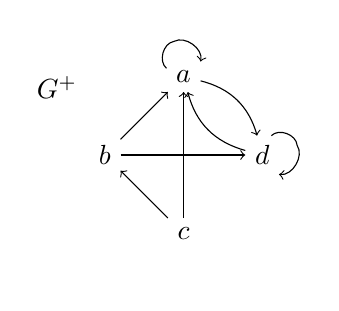
\begin{tikzpicture}
    %VARIABLES
    \pgfmathsetmacro{\gsize}{1};
    \pgfmathsetmacro{\gnum}{4};

    \foreach[count=\i] \element in {a,b,c,d} { %domain
        \node (\element) at (\i * 360 / \gnum:\gsize) {$\element$};
        \node (\element-) at (\i * 360 / \gnum:\gsize + 0.5) {};
      }
    \foreach \j/\l in {b/a, b/d, c/b, c/a} { %a to b
        \draw[->] (\j) -- (\l);
      }
    \foreach \j/\l in {a/d} { %a to b AND b to a
        \draw[->] (\j) to[bend left=20 / \gsize + 10] (\l);
        \draw[->] (\l) to[bend left=20 / \gsize + 10] (\j);
      }
    \foreach \j in {a,d} { %a to a
        \draw[->] (\j) to[bend left=65] (\j-)
        to[bend left=65] (\j);
      }
    \node[anchor=east] (name) at (145:\gsize+.5) {$G^+$}; %relation name
  \end{tikzpicture}
\end{center}

\subsubsection*{Finding the Transitive Closure of a Relation $R$ on set $A$}
Repeat until no pair is added to $R$.
\begin{center}
  If there are 3 elements $x,y,z \in A$ such that $x$R$y$ and $y$R$z$ but not $x$R$z$, add $x$R$z$ to R.
\end{center}
For example:
\begin{center}
  \begin{tikzpicture}
    %VARIABLES
    \pgfmathsetmacro{\gsize}{1.5};
    \pgfmathsetmacro{\gnum}{5};

    \foreach[count=\i] \element in {a,b,c,d,e} { %domain
        \node (\element) at (\i * 360 / \gnum:\gsize) {$\element$};
        \node (\element-) at (\i * 360 / \gnum:\gsize + 0.5) {};
      }
    \foreach \j/\l in {a/b, b/e, d/e} { %a to b
        \draw[->] (\j) -- (\l);
      }
    \foreach \j/\l in {b/c} { %a to b AND b to a
        \draw[->] (\j) to[bend left=20 / \gsize + 10] (\l);
        \draw[->] (\l) to[bend left=20 / \gsize + 10] (\j);
      }
    \foreach \j in {b,e} { %a to a
        \draw[->] (\j) to[bend left=65] (\j-)
        to[bend left=65] (\j);
      }
    \node[anchor=east] (name) at (145:\gsize+.5) {Relation}; %relation name
  \end{tikzpicture}
  \quad
  \begin{tikzpicture}
    %VARIABLES
    \pgfmathsetmacro{\gsize}{1.5};
    \pgfmathsetmacro{\gnum}{5};

    \foreach[count=\i] \element in {a,b,c,d,e} { %domain
        \node (\element) at (\i * 360 / \gnum:\gsize) {$\element$};
        \node (\element-) at (\i * 360 / \gnum:\gsize + 0.5) {};
      }
    \foreach \j/\l in {a/b, b/e, d/e} { %a to b
        \draw[->] (\j) -- (\l);
      }
    \foreach \j/\l in {b/c} { %a to b AND b to a
        \draw[->] (\j) to[bend left=20 / \gsize + 10] (\l);
        \draw[->] (\l) to[bend left=20 / \gsize + 10] (\j);
      }
    \foreach \j in {b,e} { %a to a
        \draw[->] (\j) to[bend left=65] (\j-)
        to[bend left=65] (\j);
      }
    \foreach \j/\l in {a/e,c/e} { %a to b in red
        \draw[->, red] (\j) -- (\l);
      }
    \node[anchor=east] (name) at (145:\gsize+.5) {Relation with Transitive Closure}; %relation name
  \end{tikzpicture}
\end{center}
\begin{center}
  Edges added to find transitive closure are shown in red.
\end{center}

\subsection{Matrix multiplication and graph powers}
An $n \times m$ \textbf{matrix} over set $S$ is an array of elements from $S$ with $n$ rows and $m$ columns.
Each element in a matrix is called an \textit{entry}.
A \textbf{square matrix} has the same number of rows and columns.
Here are a number of example matrixes
\begin{align*}
  \begin{bmatrix}
    1  & 3  \\
    3  & -5 \\
    -2 & -2
  \end{bmatrix}
                                             &  &
  \begin{bmatrix}
    1.1  & 3.0  & -5.4 \\
    -2.2 & -2.1 & 1
  \end{bmatrix}
                                             &  &
  \begin{bmatrix}
    1 & 0 \\
    1 & 1
  \end{bmatrix}                                                                                                                          \\
  3 \times 2 \text{ matrix over } \mathbb{Z} &  & 2 \times 3 \text{ matrix over } \mathbb{Z} &  & 2 \times 2 \text{ matrix over } \{0,1\}
\end{align*}
A directed graph $G$ can be represented by a Matrix.
\begin{center}
  $n$ vertices $\rightarrow$ $n \times n$ matrix over the set \{0,1\}, called an \textbf{adjacency matrix}
\end{center}
\begin{center}
  \begin{tikzpicture}
    %VARIABLES
    \pgfmathsetmacro{\gsize}{1};
    \pgfmathsetmacro{\gnum}{3};

    \foreach[count=\i] \element in {1,2,3} { %domain
        \node (\element) at (\i * 360 / \gnum:\gsize) {$\element$};
        \node (\element-) at (\i * 360 / \gnum:\gsize + 0.5) {};
      }
    \foreach \j/\l in {3/2} { %a to b
        \draw[->] (\j) -- (\l);
      }
    \foreach \j/\l in {1/2} { %a to b AND b to a
        \draw[->] (\j) to[bend left=20 / \gsize + 10] (\l);
        \draw[->] (\l) to[bend left=20 / \gsize + 10] (\j);
      }
    \foreach \j in {} { %a to a
        \draw[->] (\j) to[bend left=65] (\j-)
        to[bend left=65] (\j);
      }
    \foreach \j/\l in {3/1} { %a to b in red
        \draw[->, red] (\j) -- (\l);
      }
  \end{tikzpicture}
  $
    \begin{bmatrix}
      0                       & 1 & 0 \\
      1                       & 0 & 0 \\
      \text{\textcolor{red}1} & 1 & 0
    \end{bmatrix}
  $
\end{center}
A \textbf{boolean matrix} is a matrix over the set \{0,1\}, and boolean addition and multiplication are used.
The \textbf{dot product} of a matrix $A$ and $B$ is defined only if \# of columns in $A$ = \# of rows in $B$
\[
  A =
  \begin{bmatrix}
    1                       & 1                       & 1                       \\
    \text{\textcolor{red}1} & \text{\textcolor{red}0} & \text{\textcolor{red}1} \\
    0                       & 1                       & 0
  \end{bmatrix}
  \qquad
  B =
  \begin{bmatrix}
    1 & 0 & \text{\textcolor{green}1} \\
    0 & 0 & \text{\textcolor{green}1} \\
    1 & 0 & \text{\textcolor{green}1}
  \end{bmatrix}
\]
\begin{center}
  \begin{tabular}{cccccc}
    {\textcolor{red}1}            &   & {\textcolor{red}0}           &   & {\textcolor{red}1}                                         \\
    $\times$ {\textcolor{green}1} &   & $\times${\textcolor{green}1} &   & $\times$ {\textcolor{green}1}                              \\
    \hhline{-~-~-}
    1                             & + & 0                            & + & 1                             & = 1 = $(A \times B)_{2,3}$
  \end{tabular}
\end{center}

\subsubsection*{Matrix Product}
\begin{itemize}
  \item denoted as $AB$ or $A \cdot B$
  \item uses a series of dot products to compute
\end{itemize}
There are a number of properties of matrix multiplication:
\begin{center}
  \begin{tabular}{rc}
    \sout{Commutative} & $AB \not = BA$                                   \\
    Associative        & $(AB)C = A(BC)$                                  \\
    Distributive       & $A(B + C) = AB + AC$                             \\
                       & $(B+C)A = BA + CA$                               \\
    Multiplicative     & $IA = A$ and $AI = A$                            \\
                       & $OA = A$ and $AO = O$                            \\
    Dimension          & $(m \times n) \cdot (n \times k) = (m \times k)$
  \end{tabular}
\end{center}
$k^{th}$ power of a matrix:
\[
  A^k = \underbrace{A \cdot A \cdots A}_{k \text{ times}}
\]

If $G$ is a digraph, $G^k$ represents all walks of length $k$ in $G$.
There is an edge from vertex $v$ to vertex $w$ in $G^k$ if and only if there is a walk of length \textit{exactly}
$k$ from $v$ to $w$ in $G$. Matrix multiplication provides a systematic way of computing $G^k$.
\begin{enumerate}
  \item Take \textit{adjacency matrix} $A$ for graph $G$
  \item Compute $A^k$ by repeated \textit{matrix multiplication}
  \item Matrix $A^k$ is the \textit{adjacency matrix} for graph $G^k$.
\end{enumerate}

\subsubsection*{Relationship between powers of a graph and the powers of its adjacency matrix}
Let $G$ be a directed graph with $n$ vertices and let $A$ be the adjacency matrix for $G$.
Then for $k \geq 1$, $A^k$ is the adjacency matrix of $G^k$,
where boolean addition and multiplication are used to compute $A^k$.
\begin{center}
  Example:
  \qquad
  \begin{tikzpicture}
    %VARIABLES
    \pgfmathsetmacro{\gsize}{1};
    \pgfmathsetmacro{\gnum}{5};


    \foreach[count=\i] \element in {a,b,c,d,e} { %domain
        \node (\element) at (\i * 360 / \gnum:\gsize) {$\element$};
        \node (\element-) at (\i * 360 / \gnum:\gsize + 0.5) {};
      }
    \foreach \j/\l in {a/b,a/d,b/e} { %a to b
        \draw[->] (\j) -- (\l);
      }
    \foreach \j/\l in {d/e} { %a to b AND b to a
        \draw[->] (\j) to[bend left=20 / \gsize + 10] (\l);
        \draw[->] (\l) to[bend left=20 / \gsize + 10] (\j);
      }
    \foreach \j in {c} { %a to a
        \draw[->] (\j) to[bend left=65] (\j-)
        to[bend left=65] (\j);
      }
    \node[anchor=east] (name) at (145:\gsize+.5) {G}; %relation name
  \end{tikzpicture}
  \qquad
  \begin{tikzpicture}
    %VARIABLES
    \pgfmathsetmacro{\gsize}{1};
    \pgfmathsetmacro{\gnum}{5};

    \foreach[count=\i] \element in {a,b,c,d,e} { %domain
        \node (\element) at (\i * 360 / \gnum:\gsize) {$\element$};
        \node (\element-) at (\i * 360 / \gnum:\gsize + 0.5) {};
      }
    \foreach \j/\l in {a/e,b/d} { %a to b
        \draw[->] (\j) -- (\l);
      }
    \foreach \j/\l in {} { %a to b AND b to a
        \draw[->] (\j) to[bend left=20 / \gsize + 10] (\l);
        \draw[->] (\l) to[bend left=20 / \gsize + 10] (\j);
      }
    \foreach \j in {c,d,e} { %a to a
        \draw[->] (\j) to[bend left=65] (\j-)
        to[bend left=65] (\j);
      }
    \node[anchor=east] (name) at (145:\gsize+.5) {G$^2$}; %relation name
  \end{tikzpicture}
  \qquad
  \begin{tikzpicture}
    %VARIABLES
    \pgfmathsetmacro{\gsize}{1};
    \pgfmathsetmacro{\gnum}{5};

    \foreach[count=\i] \element in {a,b,c,d,e} { %domain
        \node (\element) at (\i * 360 / \gnum:\gsize) {$\element$};
        \node (\element-) at (\i * 360 / \gnum:\gsize + 0.5) {};
      }
    \foreach \j/\l in {a/d,b/e} { %a to b
        \draw[->] (\j) -- (\l);
      }
    \foreach \j/\l in {e/d} { %a to b AND b to a
        \draw[->] (\j) to[bend left=20 / \gsize + 10] (\l);
        \draw[->] (\l) to[bend left=20 / \gsize + 10] (\j);
      }
    \foreach \j in {c} { %a to a
        \draw[->] (\j) to[bend left=65] (\j-)
        to[bend left=65] (\j);
      }
    \node[anchor=east] (name) at (145:\gsize+.5) {G$^3$}; %relation name
  \end{tikzpicture}
\end{center}
\[
  A =
  \begin{bmatrix}
    0 & 1 & 0 & 1 & 0 \\
    0 & 0 & 0 & 0 & 1 \\
    0 & 0 & 1 & 0 & 0 \\
    0 & 0 & 0 & 0 & 1 \\
    0 & 0 & 0 & 1 & 0
  \end{bmatrix}
  \quad
  A^2 =
  \begin{bmatrix}
    0 & 0 & 0 & 0 & 1 \\
    0 & 0 & 0 & 1 & 0 \\
    0 & 0 & 1 & 0 & 0 \\
    0 & 0 & 0 & 1 & 0 \\
    0 & 0 & 0 & 0 & 1
  \end{bmatrix}
  \quad
  A^3 =
  \begin{bmatrix}
    0 & 0 & 0 & 0 & 0 \\
    0 & 0 & 0 & 0 & 1 \\
    0 & 0 & 1 & 0 & 0 \\
    0 & 0 & 0 & 0 & 1 \\
    0 & 0 & 0 & 1 & 0
  \end{bmatrix}
\]

\subsubsection*{Matrix Sum}
\begin{itemize}
  \item denoted as $A + B$
  \item well-defined if same \# of row and \# of columns
\end{itemize}
\[
  (A+B)_{i,j} = A_{i,j} + B_{i,j} \text{ for all $i$ and $j$ in range of $A$ or $B$}
\]
For example,
\begin{center}
  \begin{tabular}{ccccc}
    \text{\textcolor{blue}0} & + & \text{\textcolor{red}1} & = & \text{\textcolor{purple}1} \\
    $
      \begin{bmatrix}
        1                        & 0 & 1 \\
        \text{\textcolor{blue}0} & 1 & 0 \\
        0                        & 0 & 1
      \end{bmatrix}
    $                        & + &
    $
      \begin{bmatrix}
        0                       & 0 & 1 \\
        \text{\textcolor{red}1} & 1 & 0 \\
        0                       & 1 & 1
      \end{bmatrix}
    $                        & = &
    $
      \begin{bmatrix}
        1                          & 0 & 1 \\
        \text{\textcolor{purple}1} & 1 & 0 \\
        0                          & 1 & 1
      \end{bmatrix}
    $                                                                                       \\
    $A$                      & + & $B$                     & = & $A+B$
  \end{tabular}
\end{center}

\subsubsection*{Addition and Graph Union}
Let $G$ and $H$ be two directed graphs with the same vertex set.
Let $A$ be adjacency matrix for $G$ and $B$ the adjacency matrix for $H$.

Then the adjacency matrix for $G \cup H = A + B$, where boolean addition is used on the entries of matrices $A$ and $B$.
\begin{center}
  \begin{tabular}{ccccc}
    \begin{tikzpicture}
      %VARIABLES
      \pgfmathsetmacro{\gsize}{1};
      \pgfmathsetmacro{\gnum}{4};

      \foreach[count=\i] \element in {1,2,3,4} { %domain
          \node (\element) at (\i * 360 / \gnum:\gsize) {$\element$};
          \node (\element-) at (\i * 360 / \gnum:\gsize + 0.5) {};
        }
      \foreach \j/\l in {2/4,3/2} { %a to b
          \draw[->] (\j) -- (\l);
        }
      \foreach \j/\l in {1/2} { %a to b AND b to a
          \draw[->] (\j) to[bend left=20 / \gsize + 10] (\l);
          \draw[->] (\l) to[bend left=20 / \gsize + 10] (\j);
        }
      \foreach \j in {4} { %a to a
          \draw[->] (\j) to[bend left=65] (\j-)
          to[bend left=65] (\j);
        }
    \end{tikzpicture} & $\cup$ &
    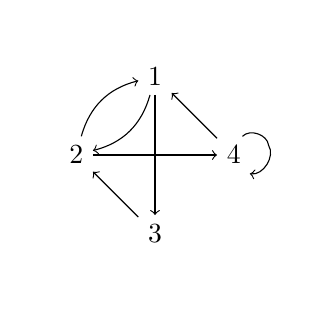
\begin{tikzpicture}
      %VARIABLES
      \pgfmathsetmacro{\gsize}{1};
      \pgfmathsetmacro{\gnum}{4};

      \foreach[count=\i] \element in {1,2,3,4} { %domain
          \node (\element) at (\i * 360 / \gnum:\gsize) {$\element$};
          \node (\element-) at (\i * 360 / \gnum:\gsize + 0.5) {};
        }
      \foreach \j/\l in {1/3,2/4,3/2,4/1} { %a to b
          \draw[->] (\j) -- (\l);
        }
      \foreach \j/\l in {1/2} { %a to b AND b to a
          \draw[->] (\j) to[bend left=20 / \gsize + 10] (\l);
          \draw[->] (\l) to[bend left=20 / \gsize + 10] (\j);
        }
      \foreach \j in {4} { %a to a
          \draw[->] (\j) to[bend left=65] (\j-)
          to[bend left=65] (\j);
        }
    \end{tikzpicture} & =      &
    \begin{tikzpicture}
      %VARIABLES
      \pgfmathsetmacro{\gsize}{1};
      \pgfmathsetmacro{\gnum}{4};

      \foreach[count=\i] \element in {1,2,3,4} { %domain
          \node (\element) at (\i * 360 / \gnum:\gsize) {$\element$};
          \node (\element-) at (\i * 360 / \gnum:\gsize + 0.5) {};
        }
      \foreach \j/\l in {4/1,3/2,1/3} { %a to b
          \draw[->] (\j) -- (\l);
        }
      \foreach \j/\l in {1/2} { %a to b AND b to a
          \draw[->] (\j) to[bend left=20 / \gsize + 10] (\l);
          \draw[->] (\l) to[bend left=20 / \gsize + 10] (\j);
        }
      \foreach \j in {4} { %a to a
          \draw[->] (\j) to[bend left=65] (\j-)
          to[bend left=65] (\j);
        }
    \end{tikzpicture}                                  \\
    $G$                                                                           & $\cup$ & $H$ & = & $G \cup H$ \\
    $A$                                                                           & +      & $B$ & = & $A+B$      \\
    $
      \begin{bmatrix}
        0 & 1 & 0 & 0 \\
        1 & 0 & 0 & 1 \\
        0 & 1 & 0 & 0 \\
        0 & 0 & 0 & 1 \\
      \end{bmatrix}
    $                                                                             & +      &
    $
      \begin{bmatrix}
        0 & 1 & 1 & 0 \\
        0 & 0 & 0 & 1 \\
        0 & 1 & 0 & 0 \\
        1 & 0 & 0 & 0 \\
      \end{bmatrix}
    $                                                                             & =      &
    $
      \begin{bmatrix}
        0 & 1 & 1 & 0 \\
        1 & 0 & 0 & 1 \\
        0 & 1 & 0 & 0 \\
        1 & 0 & 0 & 1 \\
      \end{bmatrix}
    $
  \end{tabular}
\end{center}
For digraph $G$ and adjacency matrix $A$ for $G$:
\begin{align*}
  G^+ & = G^1 \cup G^2 \cup G^3 \cup \cdots \cup G^n \\
  A^+ & = A^1 + A^2 + A^3 + \cdots + A^n
\end{align*}

\subsubsection*{Condition for well-defined matrix multiplication}
$A_{m \times n} \times B_{s \times t}$ is only defined when $n = s$, and $A \times B$ has dimensions $m \times t$.
For example:
\[
  A_{3 \times 3}
  \begin{bmatrix}
    0 & 2 & 3 \\
    1 & 0 & 1 \\
    2 & 0 & 1
  \end{bmatrix}
  \times
  B_{3 \times 1}
  \begin{bmatrix}
    1 \\
    2 \\
    0
  \end{bmatrix}
  =
  (A \times B)_{3 \times 1}
  \begin{bmatrix}
    5 \\
    4 \\
    0
  \end{bmatrix}
\]

\subsection{Partial orders}

A relation on set $A$ is a \textbf{partial order} if it is:
\begin{itemize}
  \item reflexive
  \item transitive
  \item anti-symmetric
\end{itemize}
Notation:\quad $a \preceq b$ used to express $a$R$b$

Domain along with a partial order defined on it is denoted $(A, \preceq)$
and is called a \textbf{partial ordered set} or \textbf{poset}.
\[
  \preceq \not = \leq \text{ (notice the curves)}
\]
Two elements of a poset are said to be \textit{comparable} if $x \preceq y$ or $x \succeq y$.
Otherwise they are said to be \textit{incomparable}.
A partial order is a \textit{total order} if \underline{every} two elements in the domain are \textit{comparable}.

Here is an example of a partial order:
\begin{center}
  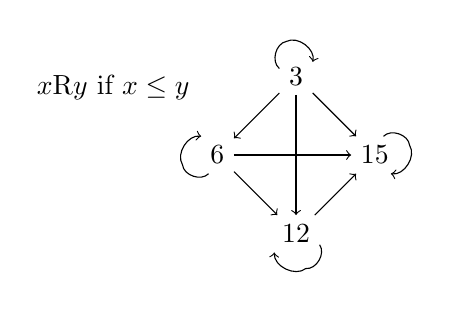
\begin{tikzpicture}
    %VARIABLES
    \pgfmathsetmacro{\gsize}{1};
    \pgfmathsetmacro{\gnum}{4};

    \foreach[count=\i] \element in {3,6,12,15} { %domain
        \node (\element) at (\i * 360 / \gnum:\gsize) {$\element$};
        \node (\element-) at (\i * 360 / \gnum:\gsize + 0.5) {};
      }
    \foreach \j/\l in {3/6,3/12,3/15,6/12,6/15,12/15} { %a to b
        \draw[->] (\j) -- (\l);
      }
    \foreach \j in {3,6,12,15} { %a to a
        \draw[->] (\j) to[bend left=65] (\j-)
        to[bend left=65] (\j);
      }
    \node[anchor=east] (name) at (145:\gsize+.5) {$x$R$y$ if $x \leq y$}; %relation name
  \end{tikzpicture}
\end{center}
\begin{itemize}
  \item An element $x$ is \textbf{minimal} element if there is no such $y \not = x$ such that $y \preceq x$
  \item An element $x$ is \textbf{maximal} element if there is no such $y \not = x$ such that $x \preceq y$
\end{itemize}

\subsubsection*{Hasse Diagram}
\begin{itemize}
  \item useful way to depict a partial order on a finite set
  \item each element is represented by a point
  \item shows relationships by placing elements that are greater than others toward the top of the diagram.
\end{itemize}
\textbf{Rules for placement and for connecting segments}
\begin{itemize}
  \item if $x \preceq y$, then make $x$ appear lower in the diagram than $y$
  \item if $x \preceq y$, and there is no such $z$ that $x \preceq z \preceq y$, then draw a segment connecting $x$ and $y$
\end{itemize}
Examples: Hasse Diagrams for a partial order on the power set of $\{1,2,3\}$, and $\{1,2,3,4,5,6\}$.
\begin{center}
  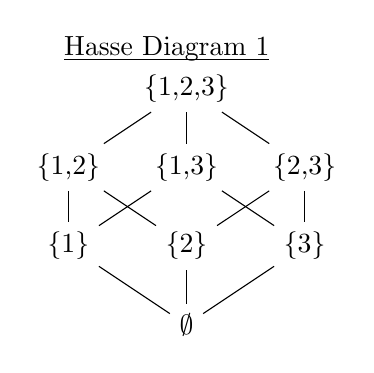
\begin{tikzpicture}
    %VARIABLES
    \pgfmathsetmacro{\spacing}{1.5};

    \foreach \rank/\elements/\size in {
    1/{{\{1,2,3\}}}/1, 2/{{\{1,2\}},{\{1,3\}},{\{2,3\}}}/3, 3/{{\{1\}},{\{2\}},{\{3\}}}/3, 4/{$\emptyset$}/1
    } {
    \foreach[count = \i] \element in \elements {
      \node (\rank-\i) at (\i * \spacing - \size / 2 * \spacing, -\rank) {\element};
    }
    }
    \foreach \j/\ls in {1-1/{2-1,2-2,2-3},2-1/{3-1,3-2},2-2/{3-1,3-3},2-3/{3-2,3-3},4-1/{3-1,3-2,3-3}} {\foreach \l in \ls {\draw (\j) -- (\l);}}
    \node (name) at (0.5,-0.5) {\underbar{Hasse Diagram 1}}; %name
  \end{tikzpicture}
  \qquad
  \begin{tikzpicture}
    %VARIABLES
    \pgfmathsetmacro{\spacing}{1.5};
    \foreach \rank/\elements/\size in {1/{6}/1, 2/{5}/1, 3/{4}/1, 4/{3}/1, 5/{2}/1, 6/{1}/1} {
    \foreach[count = \i] \element in \elements {
      \node (\rank-\i) at (\i * \spacing - \size / 2 * \spacing, -\rank) {\element};
    }
    }
    \foreach \j/\ls in {1-1/{2-1},2-1/{3-1},3-1/{4-1},4-1/{5-1},5-1/{6-1}} {\foreach \l in \ls {\draw (\j) -- (\l);}}
    \node (name) at (0.5,-0.5) {\underbar{Hasse Diagram 2}}; %name
  \end{tikzpicture}
\end{center}
The first example uses a rule of $A \preceq B \leftrightarrow A \subseteq B$,
while the second example uses a rule of $x \preceq y \leftrightarrow x \leq y$.

In general, if two elements are incomparable, then they are not connected \underline{at all} by a path of line segments
or the only paths between $x$ and $y$ require a change in direction from up to down or down to up.
Consider this partial order on the set $\{A,B,C,D,E,F,G\}$:
\begin{center}
  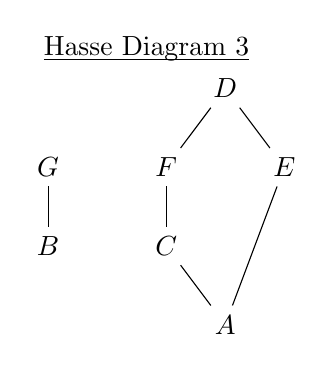
\begin{tikzpicture}
    %VARIABLES
    \pgfmathsetmacro{\spacing}{1.5};
    \foreach \rank/\elements/\size in {1/{ ,D}/2, 2/{G,F,E}/3, 3/{B,C}/3, 4/{ ,A}/2} {
    \foreach[count = \i] \element in \elements {
      \node (\element) at (\i * \spacing - \size / 2 * \spacing, -\rank) {$\element$};
    }
    }
    \foreach \j/\ls in {G/{B},D/{F,E},C/{F,A},E/{A}} {\foreach \l in \ls {\draw (\j) -- (\l);}}
    \node (name) at (0.5,-0.5) {\underbar{Hasse Diagram 3}}; %name
  \end{tikzpicture}
\end{center}
In this example, $B \preceq G$, and $A \preceq D$, but $B$ and $F$ are \underline{not} comparable.

\subsection{Strict orders and directed acyclic graphs}

\begin{itemize}
  \item Partial Order acts $\preceq$ on a domain
  \item Strict Order acts $\prec$ on a domain
\end{itemize}
A relation $R$ is a \textbf{Strict Order} if $R$ is \textit{transitive, anti-symmetric,} and \textit{anti-reflexive}.
\begin{itemize}
  \item two elements are comparable if $x \prec y$ or $x \succ y$, and otherwise incomparable
  \item strict order is a \textit{total order} if \underline{every} pair of elements is comparable
  \item element $x$ is \textbf{minimal} if no $y$ exists such that $y \prec x$
  \item element $x$ is \textbf{maximal} if no $y$ exists such that $x \prec y$
\end{itemize}
Here is an example of a strict order:
\begin{center}
  \begin{tikzpicture}
    %VARIABLES
    \pgfmathsetmacro{\gsize}{2};
    \pgfmathsetmacro{\gnum}{6};

    \foreach[count=\i] \element in {c,b,a,d,f,e} { %domain
        \node (\element) at (\i * 360 / \gnum:\gsize) {$\element$};
        \node (\element-) at (\i * 360 / \gnum:\gsize + 0.5) {};
      }
    \foreach \j/\ls in {a/{b,c,e},d/{f},b/{e},c/{e}} {\foreach \l in \ls {\draw[->] (\j) -- (\l);}}
  \end{tikzpicture}
  \qquad
  \begin{tabular}{rl}
    maximal: & $e$ and $f$ \\
    minimal: & $a$ and $d$
  \end{tabular}
\end{center}
Strict orders are also anti-symmetric. Consider a relation R that is transitive and anti-reflexive.
Then R is also anti-symmetric.

\subsubsection*{Directed Acyclic Graphs, DAGs}
A directed acyclic graph is a directed graph that has no cycles. For example, consider this DAG:
\begin{center}
  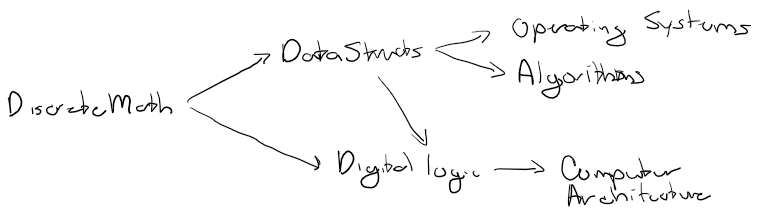
\includegraphics[width=.6\linewidth]{resources/dag prereq.png}
\end{center}
\textbf{Theorem: Directed Acyclic Graphs and Strict Orders}
Let $G$ be a directed graph. $G$ has no cycles if and only if $G^+$ is a strict order.
\begin{center}
  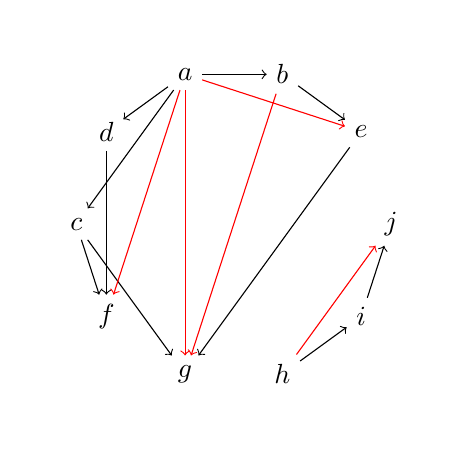
\begin{tikzpicture}
    %VARIABLES
    \pgfmathsetmacro{\gsize}{2};
    \pgfmathsetmacro{\gnum}{10};

    \foreach[count=\i] \element in {e,b,a,d,c,f,g,h,i,j} { %domain
        \node (\element) at (\i * 360 / \gnum:\gsize) {$\element$};
        \node (\element-) at (\i * 360 / \gnum:\gsize + 0.5) {};
      }
    \foreach \j/\ls in {a/{b,c,d},b/{e},c/{g,f},d/{f},e/{g},h/{i},i/{j}} {\foreach \l in \ls {\draw[->] (\j) -- (\l);}}
    \foreach \j/\ls in {a/{e,f,g},b/{g},h/{j}} {\foreach \l in \ls {\draw[->, red] (\j) -- (\l);}}
  \end{tikzpicture}
  \qquad
  \begin{tabular}{c}
    $G$ is a DAG                          \\
    Edges added by $G^+$ are shown in red \\
    Minimal: $a$ and $h$                  \\
    Maximal: $g$, $f$, and $j$
  \end{tabular}
\end{center}
Consider another example of precedence constraints for baking chocolate chip cookie:
\begin{itemize}
  \item Wash hands
  \item Grease cooking sheet
  \item Sift together dry ingredients
  \item Beat together butter and sugar
  \item Add eggs to butter and sugar
  \item Add chocolate chips
  \item Drop spoonfuls of batter onto cookie sheet and bake
\end{itemize}
Converting this into a DAG, notice how incomparable tasks can be done simultaneously by different people:
\begin{center}
  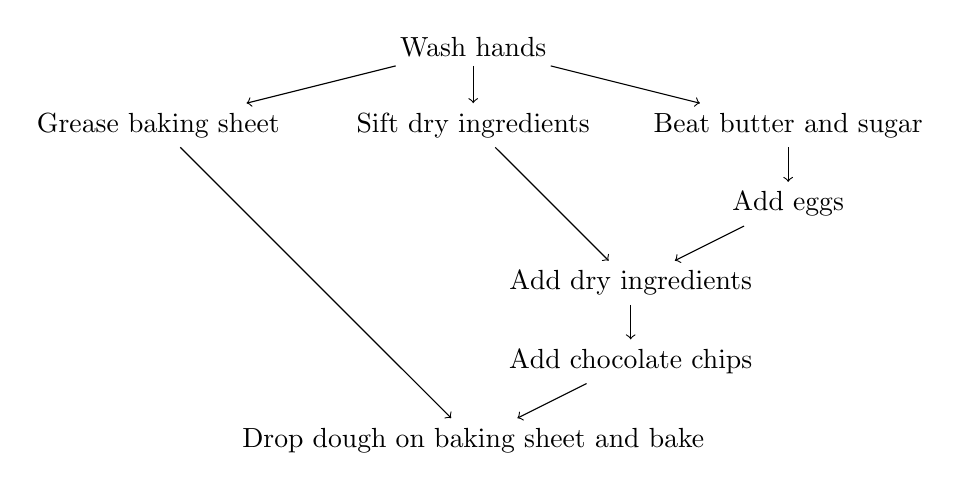
\begin{tikzpicture}
    %VARIABLES
    \pgfmathsetmacro{\spacing}{4};
    \foreach \rank/\elements/\size in {1/{Wash hands}/1, 2/{Grease baking sheet, Sift dry ingredients, Beat butter and sugar}/3,
    3/{ , , Add eggs}/3, 4/{ , Add dry ingredients}/2, 5/{ , Add chocolate chips}/2, 6/{Drop dough on baking sheet and bake}/1} {
    \foreach[count = \i] \element in \elements {\node (\element) at (\i * \spacing - \size / 2 * \spacing, -\rank) {\element};}
    }
    \foreach \j/\ls in {Wash hands/{Grease baking sheet,Sift dry ingredients,Beat butter and sugar},
    Grease baking sheet/{Drop dough on baking sheet and bake},Sift dry ingredients/{Add dry ingredients},
    Beat butter and sugar/{Add eggs},Add eggs/{Add dry ingredients},Add dry ingredients/{Add chocolate chips},
    Add chocolate chips/{Drop dough on baking sheet and bake}} {\foreach \l in \ls {\draw[->] (\j) -- (\l);}}
  \end{tikzpicture}
\end{center}

\subsubsection*{Topological Sorts of DAGs}
Consider a DAG which represents precedence constraints for a set of tasks.
Need to find an ordering which does not violate any of the precedence constraints.
A \textbf{topological} sort for a DAG is an ordering of vertices that is consistent with the edges in the graph.
\begin{itemize}
  \item If there is an edge $(u,v)$, then $u$ must appear earlier than $v$ in the topological sort.
\end{itemize}
\begin{center}
  \begin{tikzpicture}
    %VARIABLES
    \pgfmathsetmacro{\gsize}{1};
    \pgfmathsetmacro{\gnum}{3};

    \foreach[count=\i] \element in {a,b,c} {\node (\element) at (\i * 360 / \gnum:\gsize) {$\element$};}
    \foreach \j/\l in {a/c,a/b} {\draw[->] (\j) -- (\l);}
  \end{tikzpicture}
  \qquad
  \begin{tabular}{c}
    example topological sorts:         \\
    $\left\langle a,b,c\right\rangle $ \\
    $\left\langle a,c,b\right\rangle $
  \end{tabular}
\end{center}

\subsection{Equivalence relations}
A relation R is an \textbf{equivalence relation} if:
\begin{itemize}
  \item R is reflective
  \item R is transitive
  \item R is symmetric
\end{itemize}
For example:
\begin{center}
  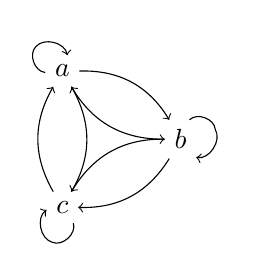
\begin{tikzpicture}
    %VARIABLES
    \pgfmathsetmacro{\gsize}{1};
    \pgfmathsetmacro{\gnum}{3};

    \foreach[count=\i] \element in {a,c,b} { %domain
        \node (\element) at (\i * 360 / \gnum:\gsize) {$\element$};
        \node (\element-) at (\i * 360 / \gnum:\gsize + 0.5) {};
        \draw[->] (\element) to[bend left=65] (\element-) to[bend left=65] (\element);
      }
    \foreach \j/\l in {a/b,b/c,a/c} { %a to b AND b to a
        \draw[->] (\j) to[bend left=20 / \gsize + 10] (\l);
        \draw[->] (\l) to[bend left=20 / \gsize + 10] (\j);
      }
  \end{tikzpicture}
  \qquad
  \begin{tikzpicture}
    %VARIABLES
    \pgfmathsetmacro{\gsize}{1};
    \pgfmathsetmacro{\gnum}{3};

    \foreach[count=\i] \element in {d,f,e} { %domain
        \node (\element) at (\i * 360 / \gnum:\gsize) {$\element$};
        \node (\element-) at (\i * 360 / \gnum:\gsize + 0.5) {};
        \draw[->] (\element) to[bend left=65] (\element-) to[bend left=65] (\element);
      }
    \foreach \j/\l in {d/f} { %a to b AND b to a
        \draw[->] (\j) to[bend left=20 / \gsize + 10] (\l);
        \draw[->] (\l) to[bend left=20 / \gsize + 10] (\j);
      }
  \end{tikzpicture}
  \qquad
  \begin{tabular}{l}
    - Reflective \\
    - Symmetric  \\
    - Transitive
  \end{tabular}
\end{center}
If $A$ is the domain of a equivalence relation and $a \in A$, then $[a]$ is called an \textbf{equivalence class},
defined to be the set of all $x \in A$, such that $a \sim x$.

For example, consider domain $\mathbb{Z}^+$ and $x \sim y$ if $x$ and $y$ have the same remainder when divided by 3.
\begin{align*}
  [0] & \text{ is } \{x \in \mathbb{Z}^+: x \mod 3 = 0\} \\
  [1] & \text{ is } \{x \in \mathbb{Z}^+: x \mod 3 = 1\} \\
  [2] & \text{ is } \{x \in \mathbb{Z}^+: x \mod 3 = 2\} \\
\end{align*}

Equivalence classes are either:
\begin{itemize}
  \item completely identical, or
  \item completely disjoint
\end{itemize}
\textbf{Theorem: Structure of Equivalence Relations}
Consider an equivalence relation on a set $A$. Let $x,y \in A$:
\begin{align*}
  \text{If}~x \sim y,~\text{then}~[x]      & = [y]                \\
  \text{If}~x \not \sim y,~\text{then}~[x] & \cap [y] = \emptyset \\
\end{align*}
\textbf{Theorem: Equivalence Relations define a Partition}
Consider and equivalence relation over a set $A$. The set of all distinct equivalence classes defines a partition of set $A$.
\begin{itemize}
  \item The term "distinct" means that if there are two equivalent classes $[a] = [b]$, then set $[a]$ is the only included one.
\end{itemize}
For example:
\begin{center}
  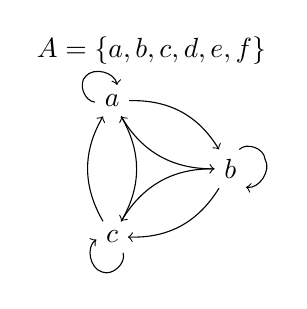
\begin{tikzpicture}
    %VARIABLES
    \pgfmathsetmacro{\gsize}{1};
    \pgfmathsetmacro{\gnum}{3};

    \foreach[count=\i] \element in {a,c,b} { %domain
        \node (\element) at (\i * 360 / \gnum:\gsize) {$\element$};
        \node (\element-) at (\i * 360 / \gnum:\gsize + 0.5) {};
        \draw[->] (\element) to[bend left=65] (\element-) to[bend left=65] (\element);
      }
    \foreach \j/\l in {a/b,b/c,a/c} { %a to b AND b to a
        \draw[->] (\j) to[bend left=20 / \gsize + 10] (\l);
        \draw[->] (\l) to[bend left=20 / \gsize + 10] (\j);
      }
    \node (name) at (90:\gsize+.5) {$A = \{a,b,c,d,e,f\}$}; %relation name
  \end{tikzpicture}
  \qquad
  \begin{tikzpicture}
    %VARIABLES
    \pgfmathsetmacro{\gsize}{1};
    \pgfmathsetmacro{\gnum}{3};

    \foreach[count=\i] \element in {d,f,e} { %domain
        \node (\element) at (\i * 360 / \gnum:\gsize) {$\element$};
        \node (\element-) at (\i * 360 / \gnum:\gsize + 0.5) {};
        \draw[->] (\element) to[bend left=65] (\element-) to[bend left=65] (\element);
      }
    \foreach \j/\l in {d/f} { %a to b AND b to a
        \draw[->] (\j) to[bend left=20 / \gsize + 10] (\l);
        \draw[->] (\l) to[bend left=20 / \gsize + 10] (\j);
      }
  \end{tikzpicture}
  \qquad
  \begin{tabular}{l}
    $[a] = \{a,b,c\}$ \\
    $[d] = \{d,f\}$   \\
    $[e] = \{e\}$     \\
  \end{tabular}
\end{center}

\subsection{N-ary relations and relational databases}
A binary relation can be generalized to more than two sets. A relation on $n$ sets is called an \textbf{N-nary Relation}.
For example:
\begin{align*}
  (w,x,y,z)  & \in \mathbb{R}^4~\text{such that}~wx=yz                                                  \\
  (3,12,4,9) & ~\text{would be in the relation because}                 & 3 \cdot 12 & = 4 \cdot 9      \\
  (3,8,5,6)  & ~\text{would \underline{not} be in the relation because} & 3 \cdot 8  & \not = 5 \cdot 6
\end{align*}

\subsubsection*{Databases}
A database is a large collection of data records that is searched and manipulated by a computer.
The \textit{regional database model} stores data records as relations.

The type of data stored in each entry of the n-tuple is called an \underline{attribute}.

A \underline{query} to a database is a request for a particular set of data.

A \underline{key} is an attribute or set of attributes that uniquely identifies each n-tuple in the databases.

For example, Airlines use the combination of flight number, date, and departure time to uniquely identify a flight.

\subsubsection*{Selection}
The \textbf{selection} operation chooses n-tuples from a relational database that satisfies particular conditions on their attributes.
For example:
\begin{center}
  \begin{tabular}{cccc}
    \# boxes & Order Date & Complete? & Client City      \\
    \hline
    8        & 6/19/2013  & NO        & Irvine           \\
    12       & 6/20/2013  & YES       & Huntington Beach \\
    15       & 6/20/2013  & YES       & Huntington Beach \\
    21       & 6/20/2013  & NO        & Irvine           \\
    3        & 6/21/2013  & NO        & Costa Mesa
  \end{tabular}
\end{center}
Search[Complete=NO]
\begin{center}
  \begin{tabular}{cccc}
    \# boxes & Order Date & Complete? & Client City \\
    \hline
    8        & 6/19/2013  & NO        & Irvine      \\
    21       & 6/20/2013  & NO        & Irvine      \\
    3        & 6/21/2013  & NO        & Costa Mesa
  \end{tabular}
\end{center}
Search[Complete=NO $\land$ Data $<$ 6/21/2013]
\begin{center}
  \begin{tabular}{cccc}
    \# boxes & Order Date & Complete? & Client City \\
    \hline
    8        & 6/19/2013  & NO        & Irvine      \\
    21       & 6/20/2013  & NO        & Irvine
  \end{tabular}
\end{center}

\subsubsection*{Projection}
The \textbf{projection} operation takes a subset of the attributes and deletes all other attributes in each of the n-tuples.
For example:
\begin{center}
  \begin{tabular}{cccc}
    \# boxes & Order Date & Complete? & Client City      \\
    \hline
    8        & 6/19/2013  & NO        & Irvine           \\
    12       & 6/20/2013  & YES       & Huntington Beach \\
    15       & 6/20/2013  & YES       & Huntington Beach \\
    21       & 6/20/2013  & NO        & Irvine           \\
    3        & 6/21/2013  & NO        & Costa Mesa
  \end{tabular}
\end{center}
Project[Order Date, Client City]
\begin{center}
  \begin{tabular}{cc}
    Order Date & Client City      \\
    \hline
    6/19/2013  & Irvine           \\
    6/20/2013  & Huntington Beach \\
    6/20/2013  & Irvine           \\
    6/21/2013  & Costa Mesa
  \end{tabular}
\end{center}
Select[Complete=NO], Project[City]
\begin{center}
  \begin{tabular}{c}
    Client City \\
    \hline
    Irvine      \\
    Costa Mesa
  \end{tabular}
\end{center}